\documentclass{article}
\usepackage{tikz}
\usetikzlibrary{positioning, fit, backgrounds, shapes.geometric, arrows.meta}
\begin{document}
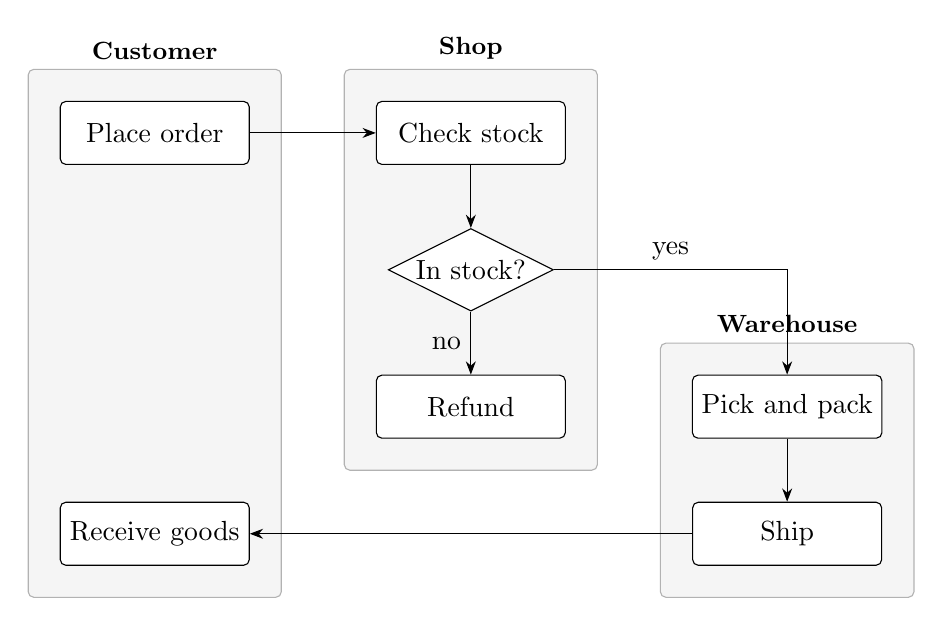
\begin{tikzpicture}[node distance=8mm and 16mm, >=Stealth,
  process/.style={draw, rounded corners=2pt, fill=white, minimum width=24mm, minimum height=8mm, align=center},
  decision/.style={draw, diamond, aspect=2, fill=white, inner sep=1pt, align=center},
  lane/.style={draw=gray!60, fill=gray!8, rounded corners=2pt, inner sep=4mm},
  lane title/.style={font=\bfseries\small}]
  \node[process] (order) {Place order};
  \node[process, right=of order] (check) {Check stock};
  \node[decision, below=of check] (instock) {In stock?};
  \node[process, below=of instock] (refund) {Refund};
  \node[process, right=of refund] (pick) {Pick and pack};
  \node[process, below=of pick] (ship) {Ship};
  \node[process] (receive) at (order |- ship) {Receive goods};

  \draw[->] (order) -- (check);
  \draw[->] (check) -- (instock);
  \draw[->] (instock) -- node[auto, swap] {no} (refund);
  \draw[->] (instock) -| node[auto, pos=0.25] {yes} (pick);
  \draw[->] (pick) -- (ship);
  \draw[->] (ship) -- (receive);

  % Lanes: each one fits its own nodes.
  \begin{scope}[on background layer]
    \node[lane, fit=(order) (receive), label={[lane title]north:Customer}] (customer) {};
    \node[lane, fit=(check) (instock) (refund), label={[lane title]north:Shop}] (shop) {};
    \node[lane, fit=(pick) (ship), label={[lane title]north:Warehouse}] (warehouse) {};
  \end{scope}
\end{tikzpicture}
\end{document}
